\documentclass[landscape, a4paper]{article}
\usepackage{pifont}
\usepackage[top=0cm, bottom=0cm, left=0cm, right=0cm]{geometry}
\usepackage{tikz}
\usepackage{hyperref}
\usetikzlibrary{patterns}
\usetikzlibrary{shapes,arrows}
\usetikzlibrary{decorations.pathreplacing, positioning}


\definecolor{anti-flashwhite}{rgb}{0.95, 0.95, 0.96}

\begin{document}
\noindent
  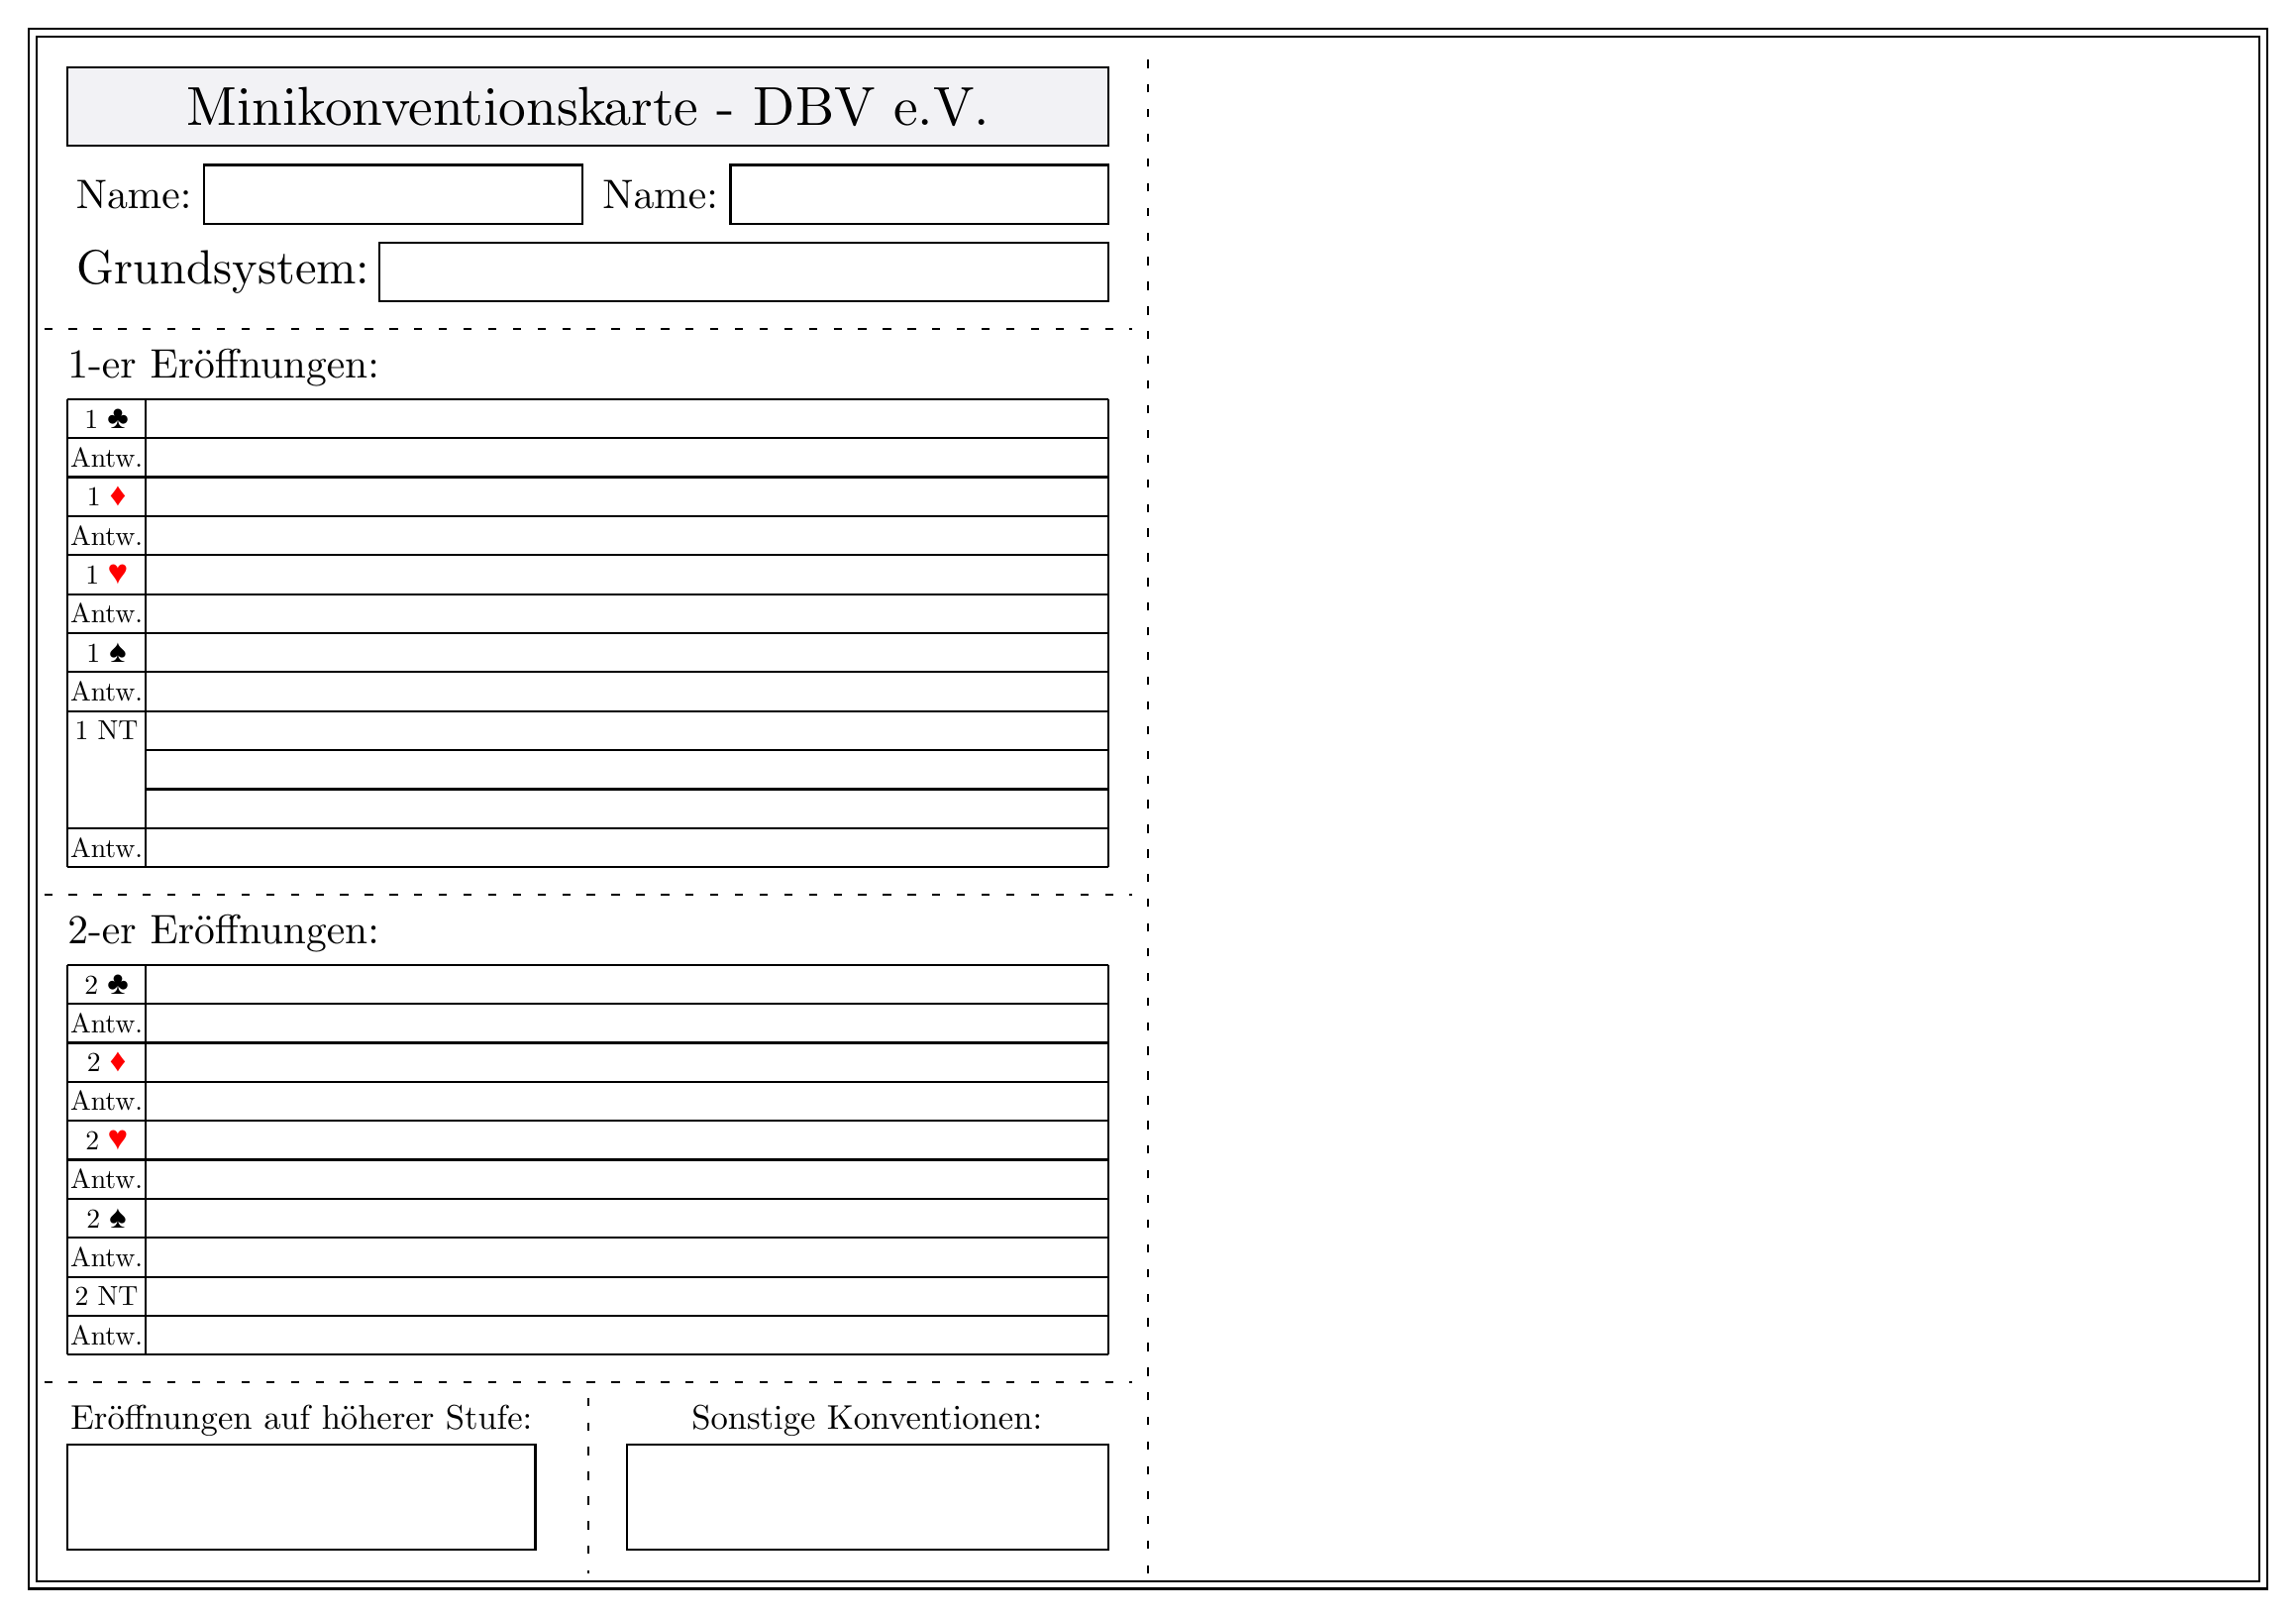
\begin{tikzpicture}

    % Border
    \draw[thick] (0cm,0cm) rectangle (28.7cm, 20.cm);
    \draw[thick] (0.1cm,0.1cm) rectangle (28.6cm, 19.9cm);

    % Separator
    \draw[thick, loosely dashed] (14.35cm, 0.2cm) -- (14.35cm, 19.8cm);

    % Heading
    \draw[thick, fill=anti-flashwhite] (0.5cm, 19.5cm) rectangle (13.85cm, 18.5cm);
    \node[very thick, scale=2] at (7.175cm, 19cm) {Minikonventionskarte - DBV e.V.};

    % Names
    \node[very thick, scale=1.5] at (1.35cm, 17.875cm) {Name:};
    \draw[thick] (2.25cm, 18.25cm) rectangle (7.1cm, 17.5cm);

    % Names
    \node[very thick, scale=1.5] at (8.1cm, 17.875cm) {Name:};
    \draw[thick] (9cm, 18.25cm) rectangle (13.85cm, 17.5cm);

    % System
    \node[very thick, scale=1.75] at (2.5cm, 16.875cm) {Grundsystem:};
    \draw[thick] (4.5cm, 17.25cm) rectangle (13.85cm, 16.5cm);

    % ------------------------------------------------------------
    % Separator
    \draw[thick, loosely dashed] (0.2cm, 16.15cm) -- (14.15cm, 16.15cm);

    % ------------------------------------------------------------
    % Opening: 1
    \node[very thick, scale=1.5] at (2.5cm, 15.65cm) {1-er Eröffnungen:};

    % Lines: Horizontal
    \foreach [evaluate=\x as \y using 15.25 - 0.5*\x] \x in {0,...,8}
      \draw[thick] (0.5cm, \y cm) -- (13.85cm, \y cm);


      \draw[thick] (1.5cm, 10.75cm) -- (13.85cm, 10.75cm);
      \draw[thick] (1.5cm, 10.25cm) -- (13.85cm, 10.25cm);
      \draw[thick] (0.5cm, 9.75cm) -- (13.85cm, 9.75cm);
      \draw[thick] (0.5cm, 9.25cm) -- (13.85cm, 9.25cm);

    % Lines: Vertikal
    \foreach [evaluate=\x as \y using 0.5 +\x] \x in {0,1, 13.35}
      \draw[thick] (\y cm, 15.25cm) -- (\y cm, 9.25cm);

    % Suits
    \node[very thick] at (1cm, 15cm) {1 \ding{168}};
    \node[very thick] at (1cm, 14.5cm) {Antw.};

    \node[very thick] at (1cm, 14cm) {1 \textcolor{red}{\ding{169}}};
    \node[very thick] at (1cm, 13.5cm) {Antw.};

    \node[very thick] at (1cm, 13cm) {1 \textcolor{red}{\ding{170}}};
    \node[very thick] at (1cm, 12.5cm) {Antw.};

    \node[very thick] at (1cm, 12cm) {1 \ding{171}};
    \node[very thick] at (1cm, 11.5cm) {Antw.};

    \node[very thick] at (1cm, 11cm) {1 NT};
    \node[very thick] at (1cm, 9.5cm) {Antw.};

    % ------------------------------------------------------------
    % Separator
    \draw[thick, loosely dashed] (0.2cm, 8.9cm) -- (14.15cm, 8.9cm);

    % ------------------------------------------------------------
    % Opening: 2
    \node[very thick, scale=1.5] at (2.5cm, 8.4cm) {2-er Eröffnungen:};

    % Lines: Horizontal
    \foreach [evaluate=\x as \y using 8 - 0.5*\x] \x in {0,...,10}
      \draw[thick] (0.5cm, \y cm) -- (13.85cm, \y cm);

    % Lines: Vertikal
    \foreach [evaluate=\x as \y using 0.5 +\x] \x in {0,1, 13.35}
      \draw[thick] (\y cm, 8cm) -- (\y cm, 3cm);

    % Suits
    \node[very thick] at (1cm, 7.75cm) {2 \ding{168}};
    \node[very thick] at (1cm, 7.25cm) {Antw.};

    \node[very thick] at (1cm, 6.75cm) {2 \textcolor{red}{\ding{169}}};
    \node[very thick] at (1cm, 6.25cm) {Antw.};

    \node[very thick] at (1cm, 5.75cm) {2 \textcolor{red}{\ding{170}}};
    \node[very thick] at (1cm, 5.25cm) {Antw.};

    \node[very thick] at (1cm, 4.75cm) {2 \ding{171}};
    \node[very thick] at (1cm, 4.25cm) {Antw.};

    \node[very thick] at (1cm, 3.75cm) {2 NT};
    \node[very thick] at (1cm, 3.25cm) {Antw.};

    % ------------------------------------------------------------
    % Separator
    \draw[thick, loosely dashed] (0.2cm, 2.65cm) -- (14.15cm, 2.65cm);

    % ------------------------------------------------------------
    % Eröffnungen hohe Stufe
    \node[very thick, scale=1.25] at (3.5cm, 2.15cm) {Eröffnungen auf höherer Stufe:};
    \draw[thick] (0.5cm, 1.85cm) rectangle (6.5cm, 0.5cm);

    % ------------------------------------------------------------
    % Separator: Vertical
    \draw[thick, loosely dashed] (7.175cm, 2.45cm) -- (7.175cm, 0.2cm);

    % ------------------------------------------------------------
    % Sonstige Konventionen
    \node[very thick, scale=1.25] at (10.75cm, 2.15cm) {Sonstige Konventionen:};
    \draw[thick] (7.675cm, 1.85cm) rectangle (13.85cm, 0.5cm);


    \end{tikzpicture}%
\end{document}
